\documentclass[
	a4paper,
	oneside,
	BCOR = 10mm,
	DIV = 12,
	12pt,
	headings = normal,
]{scrartcl}

%%% Length calculations
\usepackage{calc}
%%%

%%% Support for color
\usepackage{xcolor}
\definecolor{lightblue}{HTML}{03A9F4}
\definecolor{red}{HTML}{F44336}
%%%

%%% Including graphics
\usepackage{graphicx}
%%%

%%% Font selection
\usepackage{fontspec}

\setromanfont{STIX Two Text}[
	SmallCapsFeatures = {LetterSpace = 8},
]

\setsansfont{IBM Plex Sans}[
	Scale = MatchUppercase,
]

\setmonofont{IBM Plex Mono}[
	Scale = MatchUppercase,
]
%%%

%%% Math typesetting
\usepackage{amsmath}

\usepackage{unicode-math}
\setmathfont{STIX Two Math}

\usepackage{IEEEtrantools}
%%%

%%% List settings
\usepackage{enumitem}
\setlist[enumerate]{
	label*      = {\arabic*.},
	left        = \parindent,
	topsep      = 0\baselineskip,
	parsep      = 0\baselineskip,
	noitemsep, % override itemsep
}
% List settings for levels 2–4
\setlist[enumerate, 2, 3, 4]{
	label*      = {\arabic*.},
	left        = 0em,
	topsep      = 0\baselineskip,
	parsep      = 0\baselineskip,
	noitemsep, % override itemsep
}

\setlist[itemize]{
	label*      = {—},
	left        = \parindent,
	topsep      = 0\baselineskip,
	parsep      = 0\baselineskip,
	itemsep     = 1\baselineskip,
	noitemsep, % override itemsep
}

\setlist[description]{
	font        = {\rmfamily\upshape\bfseries},
	topsep      = 1\baselineskip,
	parsep      = 0\baselineskip,
	itemsep     = 0\baselineskip,
}

%%%

%%% Structural elements typesetting
\setkomafont{pagenumber}{\rmfamily\upshape}
\setkomafont{disposition}{\rmfamily\bfseries}

% Sectioning
\RedeclareSectionCommand[
	beforeskip = -1\baselineskip,
	afterskip  = 1\baselineskip,
	font       = {\normalsize\bfseries\scshape},
]{section}

\RedeclareSectionCommand[
	beforeskip = -1\baselineskip,
	afterskip  = 1\baselineskip,
	font       = {\normalsize\bfseries\itshape},
]{subsection}

\RedeclareSectionCommand[
	beforeskip = -1\baselineskip,
	afterskip  = 1\baselineskip,
	font       = {\normalsize\bfseries},
]{subsubsection}

\RedeclareSectionCommand[
	beforeskip = -1\baselineskip,
	afterskip  = -0.5em,
	font       = {\normalsize\mdseries\scshape\addfontfeatures{Letters = {UppercaseSmallCaps}}},
]{paragraph}
%%%

%%% Typographic enhancements
\usepackage{microtype}
%%%

%%% Language-specific settings
\usepackage{polyglossia}
\setmainlanguage{ukrainian}
\setotherlanguages{english}
%%%

%%% Captions
\usepackage{caption}
\usepackage{subcaption}

%\DeclareCaptionLabelFormat{closing}{#2)}
%\captionsetup[subtable]{labelformat = closing}

%\captionsetup[subfigure]{labelformat = closing}

\captionsetup[table]{
	aboveskip = 0\baselineskip,
	belowskip = 0\baselineskip,
}

\captionsetup[figure]{
	aboveskip = 1\baselineskip,
	belowskip = 0\baselineskip,
}

\captionsetup[subfigure]{
	labelformat = simple,
	labelformat = brace,
	justification = RaggedRight,
	singlelinecheck = false,
}
%%%

%%% Hyphenated ragged typesetting
\usepackage{ragged2e}
%%%

%%% Table typesetting
\usepackage{booktabs}
\usepackage{longtable}

\usepackage{multirow}

\usepackage{array}
\newcolumntype{v}[1]{>{\RaggedRight\arraybackslash\hspace{0pt}}p{#1}}
\newcolumntype{b}[1]{>{\Centering\arraybackslash\hspace{0pt}}p{#1}}
\newcolumntype{n}[1]{>{\RaggedLeft\arraybackslash\hspace{0pt}}p{#1}}
%%%

%%% Drawing
\usepackage{tikz}
\usepackage{tikzscale}
\usetikzlibrary{positioning}
\usetikzlibrary{arrows.meta} % Stealth arrow tips
%%%

%%% SI units typesetting
\usepackage{siunitx}
\sisetup{
	output-decimal-marker = {,},
	exponent-product      = {\cdot},
	inter-unit-product    = \ensuremath{{} \cdot {}},
	per-mode              = symbol,
}
%%%

% Code Highlighting
\usepackage{minted}
\setmintedinline{
	style = bw,
	breaklines,
}

\newminted[bashterm]{text}{%
	autogobble,%
	breaklines,%
	style=bw,%
}

\newminted[codegeneric]{text}{%
	autogobble,%
	style=bw,%
	breaklines,%
	fontsize=\small,%
}

\newmintinline{bash}{%
}

\newmintinline[minttext]{text}{%
	breaklines,%
	breakanywhere,%
}

%%% Framing code listings
\usepackage{tcolorbox}
\tcbuselibrary{breakable}
\tcbuselibrary{minted}
\tcbuselibrary{skins}

% Text file listing
\newtcblisting[
	auto counter,
	list inside,
	number within = section,
]{listingplaintext}[3][]{%
	minted language = text,
	minted style    = bw,
	minted options  = {
		autogobble,
		linenos,
		tabsize = 4,
		breaklines,
		breakanywhere,
		fontsize = \footnotesize,
	},
	empty,
	sharp corners,
	coltitle = black,
	borderline horizontal = {1pt}{0pt}{black},
	titlerule = {0.5pt},
	titlerule style = {
		black,
	},
	toptitle = 0.3em,
	bottomtitle = 0.3em,
	before skip      = \intextsep,
	after  skip      = \intextsep,
	title            = {Лістинг \thetcbcounter: #2},
	list entry       = {\protect\numberline{\thetcbcounter}#2},
	left = 0em,
	right = 0em,
	%
	listing only,
	breakable,
	%
	label = {#3},%
}

\newtcblisting[
	use counter from = listingplaintext,
	list inside,
	number within = section,
]{listingpython}[3][]{%
	minted language = python,
	minted style    = bw,
	minted options  = {
		autogobble,
		linenos,
		tabsize = 4,
		breaklines,
		breakanywhere,
		fontsize = \footnotesize,
	},
	empty,
	sharp corners,
	coltitle = black,
	borderline horizontal = {1pt}{0pt}{black},
	titlerule = {0.5pt},
	titlerule style = {
		black,
	},
	toptitle = 0.3em,
	bottomtitle = 0.3em,
	before skip      = \intextsep,
	after  skip      = \intextsep,
	title            = {Лістинг \thetcbcounter: #2},
	list entry       = {\protect\numberline{\thetcbcounter}#2},
	left = 0em,
	right = 0em,
	%
	listing only,
	breakable,
	%
	label = {#3},
	%
	#1%
}

\newtcbinputlisting[
	use counter from = listingplaintext,
	list inside,
	number within = section
]{\inputpython}[4][]{%
	minted language = python,
	minted style    = bw,
	minted options  = {
		autogobble,
		linenos,
		tabsize = 4,
		breaklines,
		breakanywhere,
		fontsize = \footnotesize,
	},
	empty,
	sharp corners,
	coltitle = black,
	borderline horizontal = {1pt}{0pt}{black},
	titlerule = {0.5pt},
	titlerule style = {
		black,
	},
	toptitle = 0.3em,
	bottomtitle = 0.3em,
	before skip      = \intextsep,
	after  skip      = \intextsep,
	title            = {Лістинг \thetcbcounter: #3},
	list entry       = {\protect\numberline{\thetcbcounter}#3},
	left = 0em,
	right = 0em,
	%
	listing file={#2},
	listing only,
	breakable,
	%
	label = {#4}
}

% Linux command-line listing
\newtcblisting{linuxterm}%
{%
	% Syntax highlighing options
	listing only,%
	minted language = bash,%
	minted options={%
		autogobble,%
		linenos%
	},%
	% Presentation options
	empty,%
	%% Margins
	sharp corners,%
	toptitle = 0.0em,%
	bottomtitle = 0.0em,%
	left = 0em,%
	right = 0em,%
	before skip = \intextsep,%
	after skip = \intextsep,%
}

\newtcblisting{linuxtermout}%
{%
	% Syntax highlighing options
	listing only,%
	minted language = text,%
	minted options={%
		autogobble,%
		linenos%
	},%
	% Presentation options
	empty,%
	%% Margins
	sharp corners,%
	toptitle = 0.0em,%
	bottomtitle = 0.0em,%
	left = 0em,%
	right = 0em,%
	before skip = \intextsep,%
	after skip = \intextsep,%
}

% Dockerfile listings
\newtcblisting[
	use counter from = listingplaintext,
	list inside,
	number within = section,
]{listingdocker}[3][]{%
	minted language = dockerfile,
	minted style    = bw,
	minted options  = {
		autogobble,%
		linenos,
		tabsize = 4,
		breaklines,
		breakanywhere,
		fontsize = \footnotesize,
	},
	empty,
	sharp corners,
	coltitle = black,
	borderline horizontal = {1pt}{0pt}{black},
	titlerule = {0.5pt},
	titlerule style = {
		black,
	},
	toptitle = 0.3em,
	bottomtitle = 0.3em,
	before skip      = \intextsep,
	after  skip      = \intextsep,
	title            = {Лістинг \thetcbcounter: #2},
	list entry       = {\protect\numberline{\thetcbcounter}#2},
	left = 0em,
	right = 0em,
	%
	listing only,
	breakable,
	%
	label = {#3},%
}

% Docker Compose listings
\newtcblisting[
	use counter from = listingplaintext,
	list inside,
	number within = section,
]{listingdockercompose}[3][]{%
	minted language = yaml,
	minted style    = bw,
	minted options  = {
		autogobble,%
		linenos,
		tabsize = 4,
		breaklines,
		breakanywhere,
		fontsize = \footnotesize,
	},
	empty,
	sharp corners,
	coltitle = black,
	borderline horizontal = {1pt}{0pt}{black},
	titlerule = {0.5pt},
	titlerule style = {
		black,
	},
	toptitle = 0.3em,
	bottomtitle = 0.3em,
	before skip      = \intextsep,
	after  skip      = \intextsep,
	title            = {Лістинг \thetcbcounter: #2},
	list entry       = {\protect\numberline{\thetcbcounter}#2},
	left = 0em,
	right = 0em,
	%
	listing only,
	breakable,
	%
	label = {#3},%
}


% Customize minted line numbers
\renewcommand{\theFancyVerbLine}{\ttfamily\scriptsize\arabic{FancyVerbLine}}

%%%

%%% Typeset menus and keys
\usepackage{menukeys}[
	os=win,
]
%%%

%%% Links and hyperreferences
\usepackage{hyperref}
\hypersetup{
	bookmarksnumbered = true,
	colorlinks      = false,
	linkbordercolor = red,
	urlbordercolor  = lightblue,
	pdfborderstyle  = {/S/U/W 1.5},
}
%%%

%%% Length adjustment

% Set baselineskip, default is 14.5 pt
\linespread{1.068966} % ~15.5 pt
\setlength{\emergencystretch}{1em}
\setlength{\parindent}{1.5em}
\newlength{\gridunitwidth}
\setlength{\gridunitwidth}{\textwidth / 12}
%%%

%%% Custom commands
\newcommand{\allcaps}[1]{%
	{%
		\addfontfeatures{%
			Letters = UppercaseSmallCaps,
			LetterSpace = 8,%
		}%
		#1%
	}%
}
\newcommand{\filename}[1]{\texttt{#1}}
\newcommand{\progname}[1]{\texttt{#1}}
\newcommand{\commandname}[1]{\texttt{#1}}
\newcommand{\modulename}[1]{\texttt{#1}}
\newcommand{\ifname}[1]{\texttt{#1}} % typesets a network interface's name

\newcommand{\transeng}[1]{{англ.}~\textit{\textenglish{#1}}}
%%%

%%% Custom math commands
\newcommand{\longvar}[1]{\mathit{#1}}
%%%

\begin{document}

\begin{titlepage}
		\begin{center}
			Міністерство освіти і~науки України\\
			Національний авіаційний університет\\
			Факультет кібербезпеки, комп'ютерної та~програмної інженерії\\
			Кафедра комп'ютеризованих систем управління

			\vspace{\fill}
				Лабораторна робота №~1.6\\
				з~дисципліни «Захист інформації в~комп'ютерних системах»\\
				на~тему «Налаштування міжмережевих екранів»

			\vspace{\fill}

			\begin{flushright}
				Виконав:\\
				студент \allcaps{ФККПІ}\\
				групи \allcaps{СП}-425\\
				Клокун В.\,Д.\\
				Перевірила:\\
				Супрун О.\,М.
			\end{flushright}

			Київ 2019
		\end{center}
	\end{titlepage}

	\section{Мета роботи}
		Ознайомитись з~основними принципами функціонування міжмережевих екранів та їх настроювання.

	\section{Завдання роботи}
		Встановити та настроїти програмне забезпечення міжмережевого екрану; сконфігурувати програмне забезпечення~\progname{\textenglish{iptalbes}} для раціональної обробки мережевих пакетів.

	\section{Хід~роботи}
		Щоб розпочати роботу, необхідно встановити програму~\progname{\textenglish{gufw}}~— інтерфейс для програми~\progname{\textenglish{iptables}}. Для цього виконуємо таку команду:
		\begin{codegeneric}
			sudo apt install gufw
		\end{codegeneric}
		Коли команда завершить роботу, в операційній системі буде встановлена програма~\progname{\textenglish{gufw}}. Розглянемо встановлену програму. Для цього запустимо її і ознайомимось з інтерфейсом~(рис.~\ref{fig:01-gufw}).

		\begin{figure}[!htbp]
			\begin{subfigure}[b]{3 \gridunitwidth - 1em / 4}
				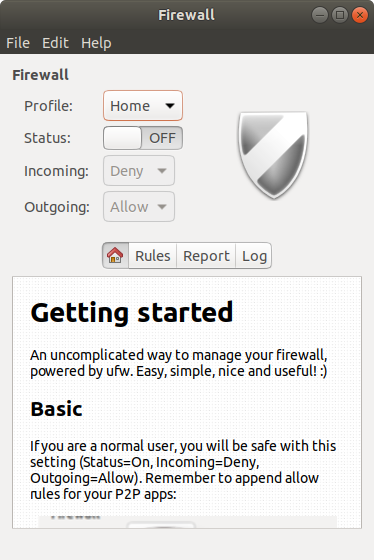
\includegraphics[width = \columnwidth]{./assets/01.png}
				\caption{}
				\label{subfig:01-01}
			\end{subfigure}%
			\hspace{0.333333em}%
			\begin{subfigure}[b]{3 \gridunitwidth - 1em / 4}
				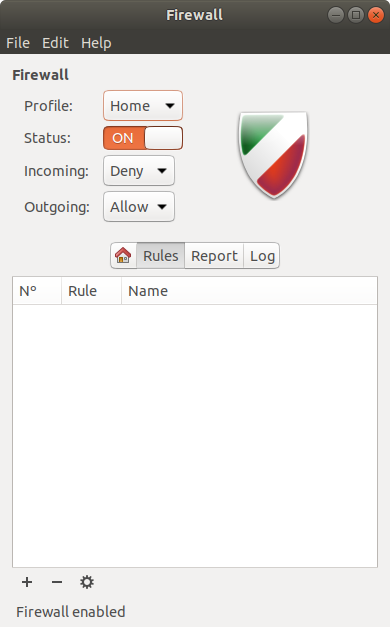
\includegraphics[width = \columnwidth]{./assets/02.png}
				\caption{}
				\label{subfig:01-02}
			\end{subfigure}%
			\hspace{0.333333em}%
			\begin{subfigure}[b]{3 \gridunitwidth - 1em / 4}
				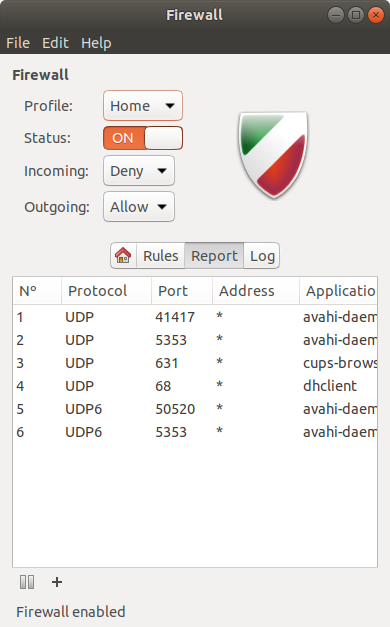
\includegraphics[width = \columnwidth]{./assets/03.png}
				\caption{}
				\label{subfig:01-03}
			\end{subfigure}%
			\hspace{0.333333em}%
			\begin{subfigure}[b]{3 \gridunitwidth - 1em / 4}
				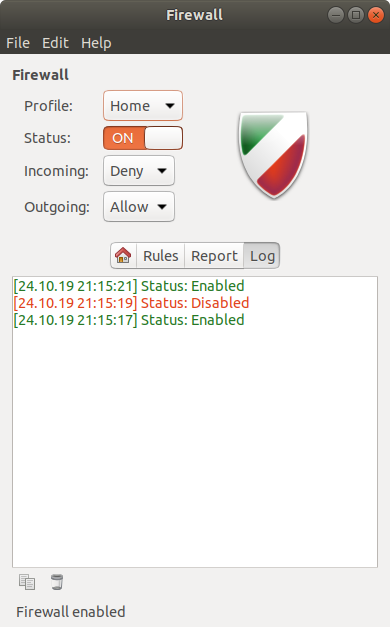
\includegraphics[width = \columnwidth]{./assets/04.png}
				\caption{}
				\label{subfig:01-04}
			\end{subfigure}%
			\caption{Інтерфейс програми~\progname{\textenglish{gufw}}}
			\label{fig:01-gufw}
		\end{figure}

		Основними елементами головного вікна програми є чотири вікна: «Домашня сторінка», «Правила», «Звіт» та «Логи». На домашній сторінці розказано, як користуватись програмою. Вкладка «Правила» містить правила міжмережевого екрана. На вкладці «Звіт» показані вхідні підключення, які намагались встановити ззовні. На вкладці «Логи» міститься інформація про роботу з міжмережевим екраном: включення, виключення, зміни правил та інші події.

		Щоб перевірити роботу встановленого інтерфейсу до міжмережевого екрану, створимо правило, яка блокуватиме вихідні підключення до~вузла з~\textenglish{\allcaps{IP}}-адресою 8.8.8.8~(рис.~\ref{fig:02}).

		\begin{figure}[!htbp]
			\begin{subfigure}[b]{7 \gridunitwidth - 1em / 2}
				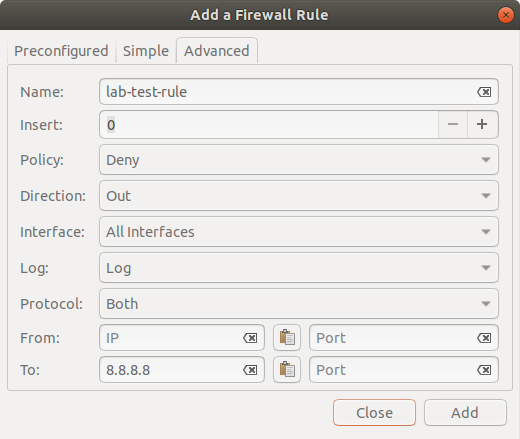
\includegraphics[width = \columnwidth]{./assets/09.png}
				\caption{}
				\label{subfig:02-01}
			\end{subfigure}%
			\hspace{1em}%
			\begin{subfigure}[b]{5 \gridunitwidth - 1em / 2}
				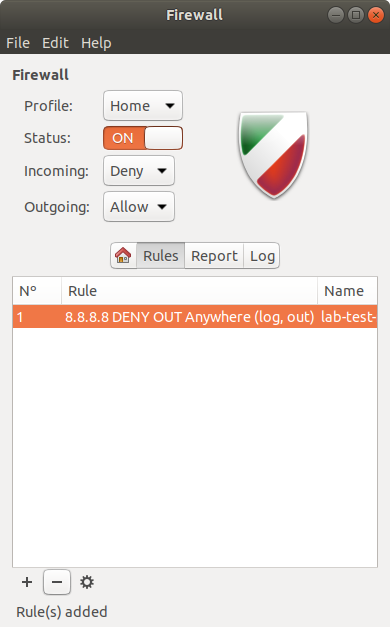
\includegraphics[width = \columnwidth]{./assets/10.png}
				\caption{}
				\label{subfig:02-02}
			\end{subfigure}
			\begin{subfigure}[b]{9 \gridunitwidth - 1em / 2}
				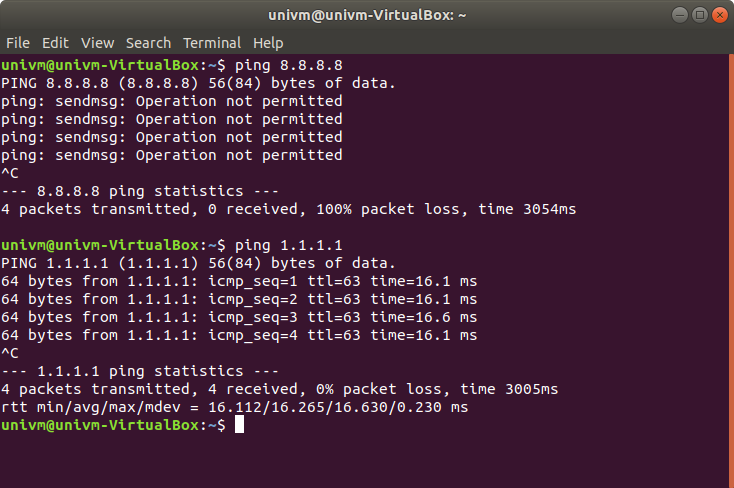
\includegraphics[width = \columnwidth]{./assets/11.png}
				\caption{}
				\label{subfig:02-03}
			\end{subfigure}%
			\caption{Створення правила для міжмережевого екрана у програмі~\progname{\textenglish{gufw}}}
			\label{fig:02}
		\end{figure}

		Після створення правила спроба підключитись до заблокованого вузла відхиляється і закінчується невдачею, а для дозволеного виконується успішно.

		Видалимо правило і перевіримо, чи можна тепер підключитись до раніше заблокованого вузла. Як бачимо, після видалення правила підключення проходить успішно~(рис.~\ref{fig:03}).

		\begin{figure}[!htbp]
			\begin{subfigure}[b]{4 \gridunitwidth - 1em / 2}
				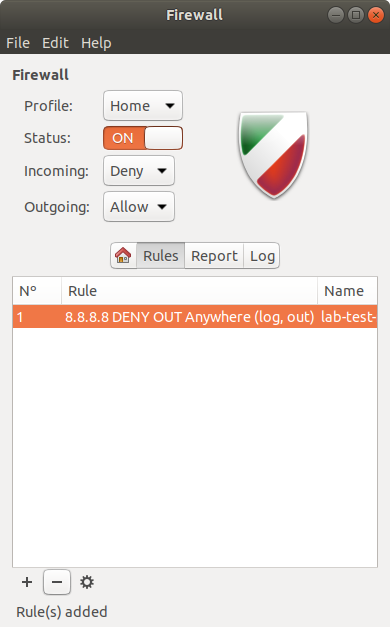
\includegraphics[width = \columnwidth]{./assets/10.png}
				\caption{}
				\label{subfig:03-01}
			\end{subfigure}%
			\hspace{1em}%
			\begin{subfigure}[b]{8 \gridunitwidth - 1em / 2}
				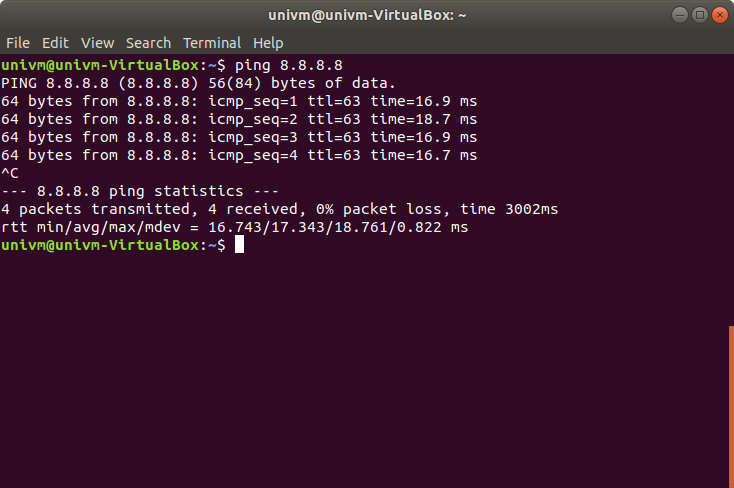
\includegraphics[width = \columnwidth]{./assets/12.png}
				\caption{}
				\label{subfig:03-02}
			\end{subfigure}%
			\caption{Спроба підключення після видалення правила у~програмі~\progname{\textenglish{gufw}}}
			\label{fig:03}
		\end{figure}

		Перевіривши справність роботи правил, переглянемо, які правила діють у міжмережевому екрані на даний момент. Для цього виконаємо таку команду:
		\begin{codegeneric}
			sudo iptables -L
		\end{codegeneric}
		Після завершення роботи команди на екран будуть виведені усі правила, знайдені у налаштуваннях міжмережевого екрана~(рис.~\ref{fig:04}).

		\begin{figure}[!htbp]
			\centering
			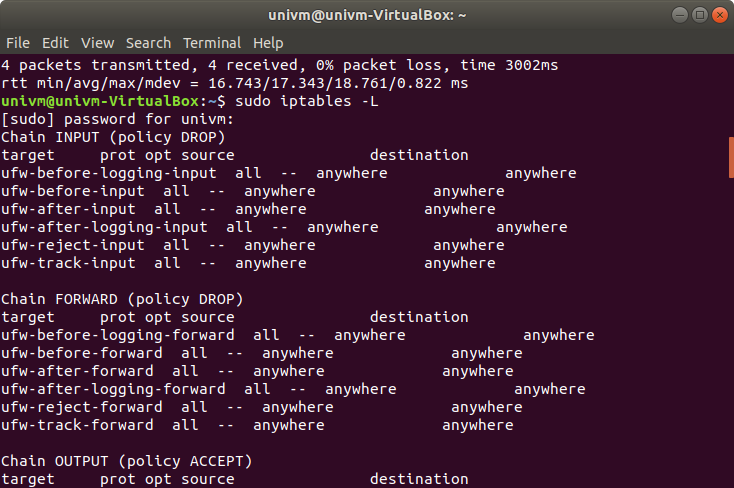
\includegraphics[width = 6 \gridunitwidth]{./assets/13.png}
			\caption{Список активних правил міжмережевого екрана}
			\label{fig:04}
		\end{figure}

		Отже, тепер ми навчились працювати з міжмережевим екраном за допомогою графічного інтерфейсу~\progname{\textenglish{gufw}}. Переходимо до налаштування міжмережевого екрану на комп'ютері під управлінням операційної системи~\textenglish{Windows}.

		В операційній системі~\textenglish{Windows} міжмережевий екран прийнято називати «брандмауером». Щоб його налаштувати, необхідно відкрити Панель керування і обрати елемент~«Брандмауер~\textenglish{Windows}», а потім у боковому меню натиснути на надпис~«Додаткові параметри». В результаті відкриється вікно налаштувань брандмауера~(рис.~\ref{fig:05}).

		\begin{figure}[!htbp]
			\centering
			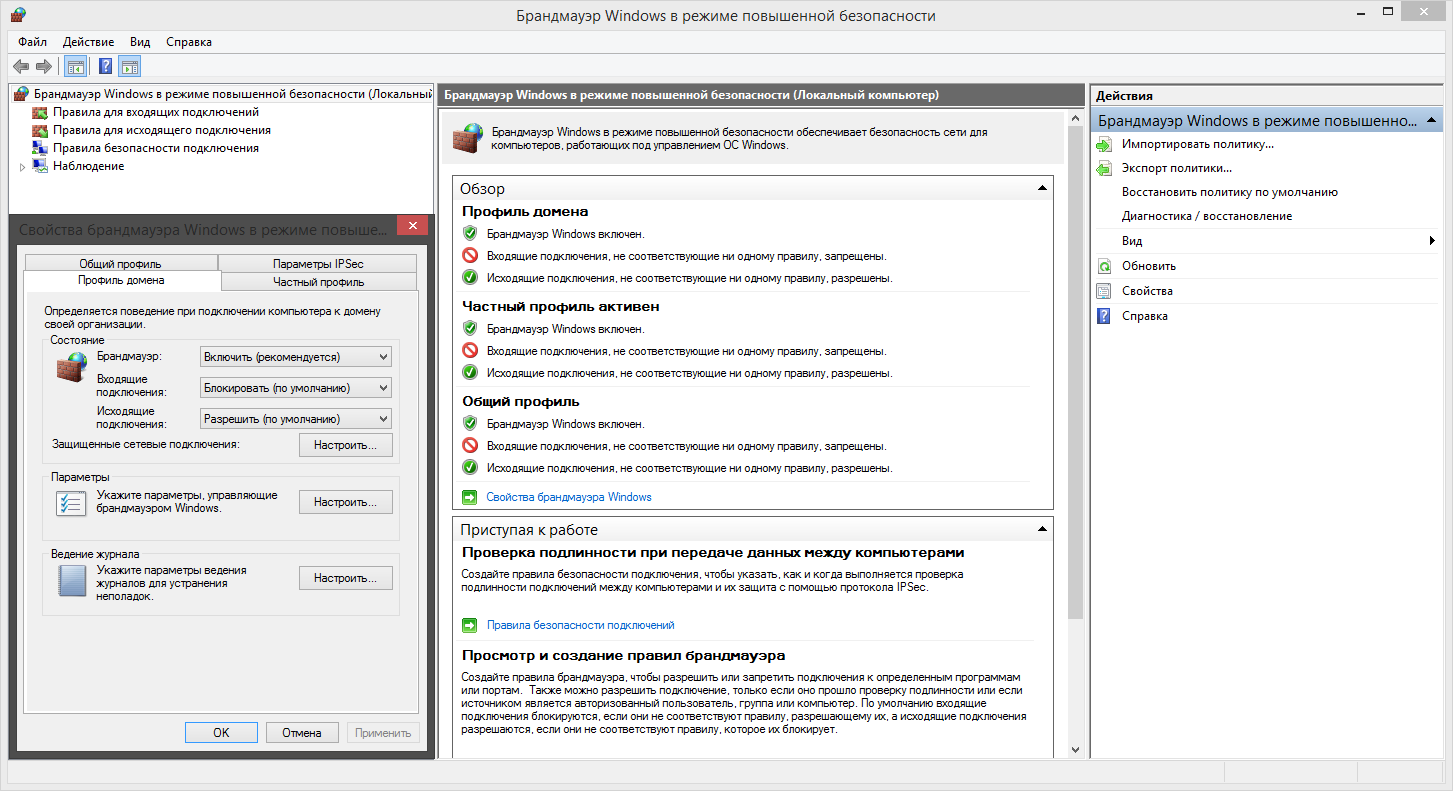
\includegraphics[width = 9 \gridunitwidth]{./assets/14-01.png}
			\caption{Вікно налаштування брандмауера~\textenglish{Windows}}
			\label{fig:05}
		\end{figure}

		У з'явившомуся вікні вмикаємо брандмауер для поточного домену, приватного та загального профілів і підтверджуємо вибрані налаштування. Після цього брандмауер налаштований. Перевіримо його роботу. Для цього спробуємо підключитись від імені комп'ютера під управлінням операційної системи~\textenglish{\allcaps{GNU}/Linux} до комп'ютера під управлінням~\textenglish{Windows} спочатку коли брандмауер увімкнений, а потім~— вимкнений~(рис.~\ref{fig:06}).

		\begin{figure}[!htbp]
			\begin{subfigure}[b]{7 \gridunitwidth - 1em / 2}
				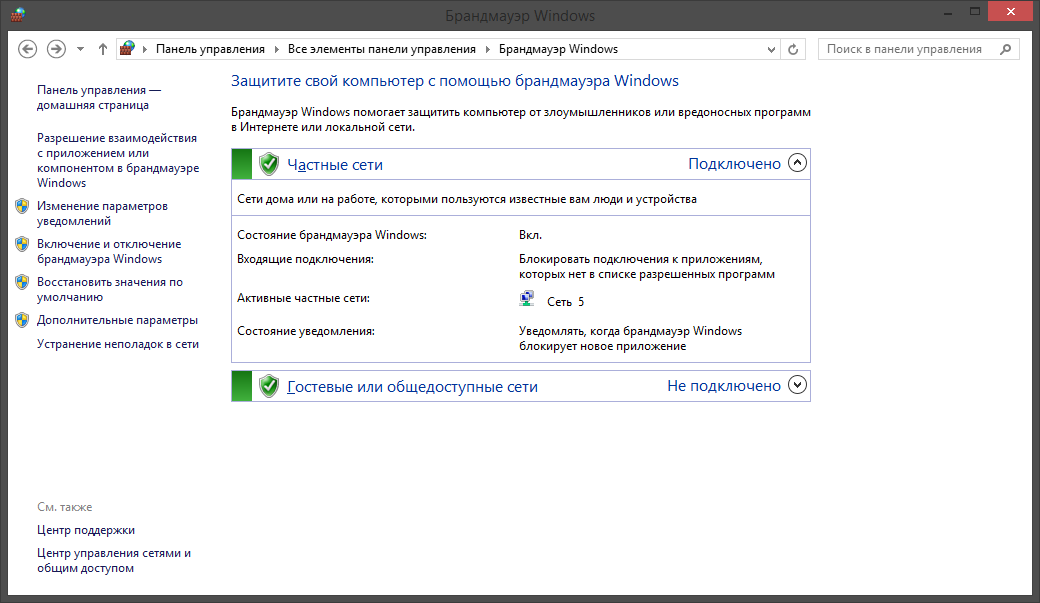
\includegraphics[width = \columnwidth]{./assets/14-02.png}
				\caption{}
				\label{subfig:06-01}
			\end{subfigure}%
			\hspace{1em}%
			\begin{subfigure}[b]{5 \gridunitwidth - 1em / 2}
				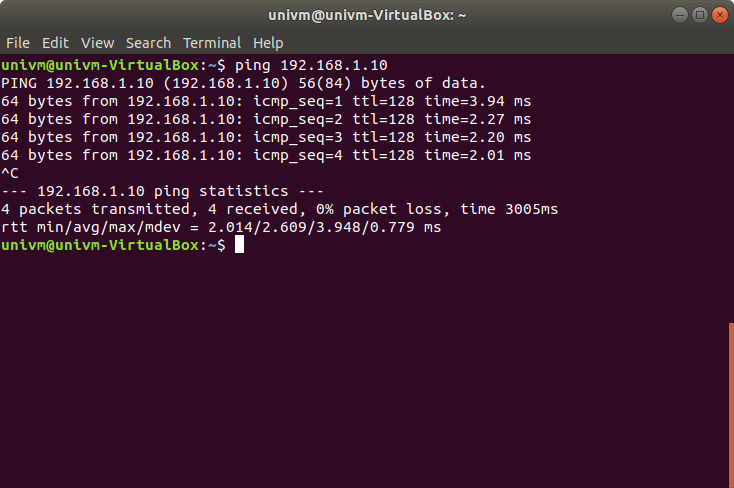
\includegraphics[width = \columnwidth]{./assets/14-03.png}
				\caption{}
				\label{subfig:06-02}
			\end{subfigure}
			\begin{subfigure}[b]{7 \gridunitwidth - 1em / 2}
				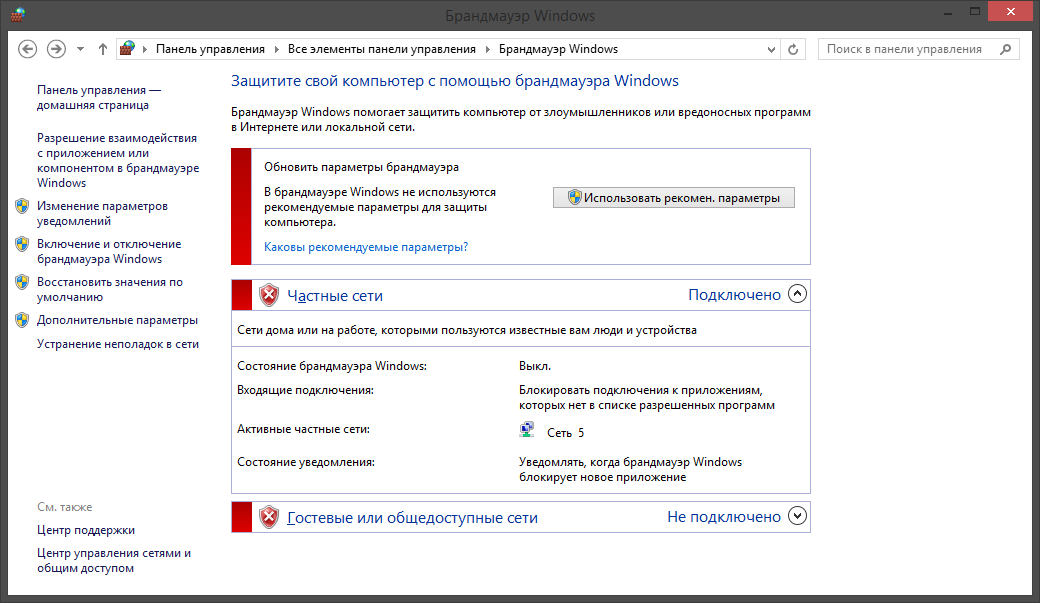
\includegraphics[width = \columnwidth]{./assets/14-04.png}
				\caption{}
				\label{subfig:06-03}
			\end{subfigure}
			\hspace{1em}%
			\begin{subfigure}[b]{5 \gridunitwidth - 1em / 2}
				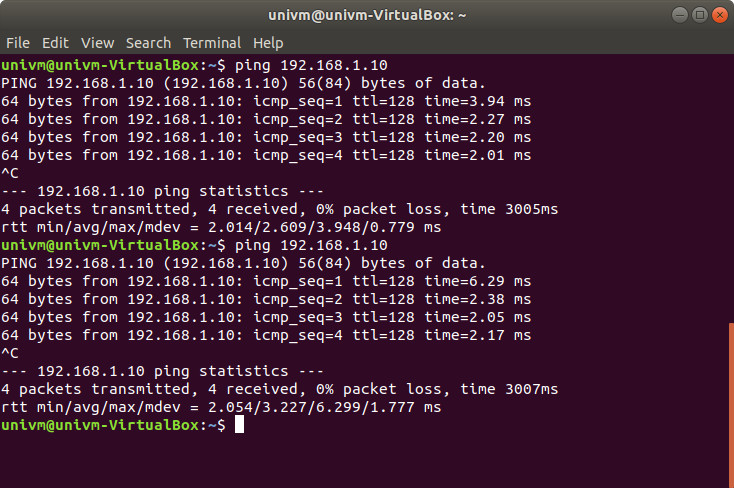
\includegraphics[width = \columnwidth]{./assets/14-05.png}
				\caption{}
				\label{subfig:06-04}
			\end{subfigure}%
			\caption{Спроби підключення до комп'ютера під управлінням~\textenglish{Windows} з різними налаштуваннями брандмауера}
			\label{fig:06}
		\end{figure}

		Отже, ми ознайомились з можливостями, особливостями і налаштуваннями міжмережевого екрана в операційній системі~\textenglish{Windows}.

		Повернемось до міжмережевого екрана в операційній системі~\textenglish{\allcaps{GNU}/Linux}. Вимкнемо правила, встановлені програмою~\progname{\textenglish{gufw}} і переглянемо активні правила, які залишились~(рис.~\ref{fig:07}).

		\begin{figure}[!htbp]
			\centering
			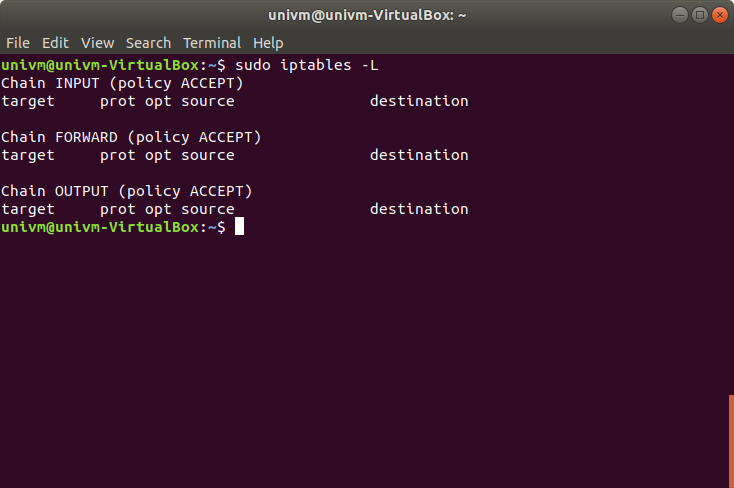
\includegraphics[width = 7 \gridunitwidth]{./assets/15.png}
			\caption{Активні правила міжмережевого екрана за замовчуванням}
			\label{fig:07}
		\end{figure}

		Заблокуємо вхідні, вихідні і транзитні пакети, тобто зробимо так, щоб жоден пакет не проходив через мережеві інтерфейси. Для цього виконаємо такі команди:
		\begin{codegeneric}
			iptables -P INPUT DROP
			iptables -P OUTPUT DROP
			iptables -P FORWARD DROP
		\end{codegeneric}
		В результаті виконання команди всі пакети будуть заблоковані і жоден не зможе пройти крізь будь-який мережевий інтерфейс. За умовами завдання збережемо поточні правила міжмережевого екрана. Для цього виконаємо таку команду:
		\begin{codegeneric}
			sudo iptables-save > uni/iptables-01.txt
		\end{codegeneric}
		Після того, як правила збережені, переглянемо список активних правил і переконаємось у цьому на практиці~(рис.~\ref{fig:08}).

		\begin{figure}[!htbp]
			\begin{subfigure}[b]{6 \gridunitwidth - 1em / 2}
				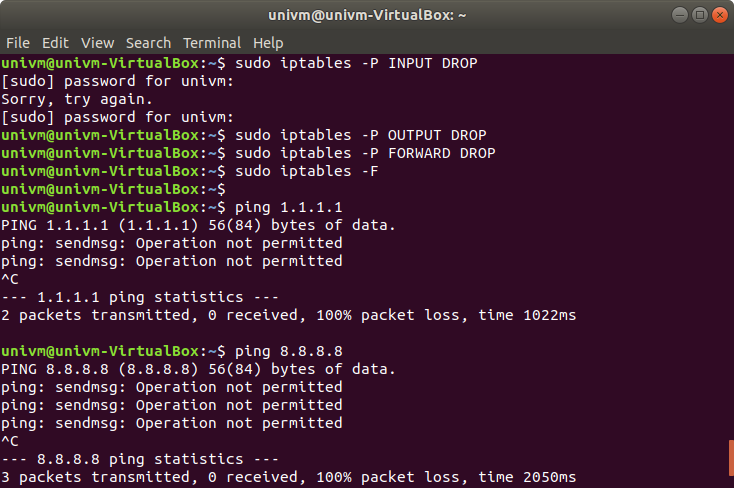
\includegraphics[width = \columnwidth]{./assets/17.png}
				\caption{}
				\label{subfig:08-01}
			\end{subfigure}%
			\hspace{1em}%
			\begin{subfigure}[b]{6 \gridunitwidth - 1em / 2}
				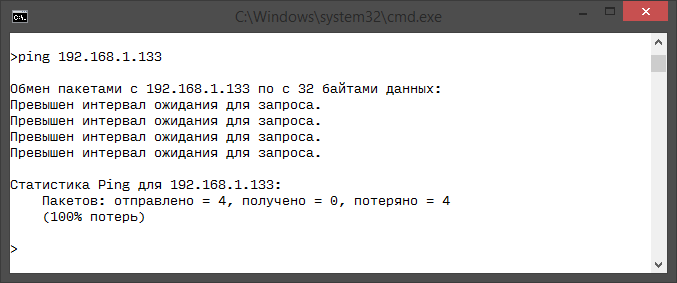
\includegraphics[width = \columnwidth]{./assets/18.png}
				\caption{}
				\label{subfig:08-02}
			\end{subfigure}
			\caption{Спроби підключення до комп'ютера під управлінням~\textenglish{\allcaps{GNU}/Linux} із повною забороною пропуску пакетів}
			\label{fig:08}
		\end{figure}

		Як бачимо, ні внутрішні, ні зовнішні пакети не можуть пройти крізь мережеві інтерфейси комп'ютера, в якому міжмережевий екран налаштований на відторгнення усіх пакетів.

		Зазвичай~\progname{\textenglish{iptables}} використовують з ключем~\verb|-P|, який позначає створення нової політики міжмережевого екрану. Також використовують ключ~\verb|-L|, щоб вивести список усіх активних правил, а також ключ~\verb|-F|, щоб очистити і оновити усі активні правила міжмережевого екрана.

	\section{Висновок}
		Виконуючи дану лабораторну роботу, ми~ознайомились з~основними принципами функціонування міжмережевих екранів та їх настроювання.

\end{document}
